\chapter{Results}

In this chapter the main results of the numerical investigation of the Bose-Hubbard superfluid to Mott-insulator phase transition are presented.

The framework set up for performing optimal control of lattice systems consist of multiple components working together:\\
The quantum state of the system is parametrized as a Matrix Product State (see Chapter \ref{chap:MPS}), whereby the exponential scaling of the Hilbert space with system size can be avoided. For time evolving the state a version of the tDMRG algorithm is employed (see Section \ref{sec:modTMDRG}), which is modified to accommodate some of the difficulties otherwise associated with the control problem.
Quantum optimal control determines the best way to manipulate a set of external parameters in order to facilitate a state transfer $\ket{\psi_0} \to \ket{\psi_{\mathrm{target}}}$. These states are calculated initially using the DMRG algorithm (see Section \ref{sec:DMRG}) at the fixed control points $\boldsymbol{u}(0)$ and $\boldsymbol{u}(T)$, such that these states are guaranteed to be the ground state. Most of the tensor operations used are implemented in the ITensor library \cite{ITensor}.
The optimal set of control parameters needed for completing the state transfer with the highest possible fidelity is calculated using the GROUP algorithm described in Section \ref{sec:GROUP}. In each iteration of GROUP, the gradient of the cost functional is calculated and used to update the control through the Interior Point method (see Section \ref{sec:IntPoint}). The Interior Point method is implemented in IPOPT library \cite{Wachter2006}.\\


explain how chapter is ordered/which things are examined



\section{Characterization of Methods on a Small System}

\subsection{Boundary Conditions}
Section \ref{sec:BHmodel} describes how the Bose-Hubbard model is only well defined within the tight-binding limit. This is especially an issue for lattice depth below the limit, as the Wannier functions may start overlapping with the next-nearest neighbouring sites, thus facilitating two-site hopping, which is not accounted for in the model. Thus, the starting value of the control must be chosen with care. In \cite{FrankBloch,Doria2011} initial lattice depths at $V_0 (0) = 3 E_r$ and lower were chosen, where it was argued that the model is still a decent approximation at this depth. Hence, an initial control of $U/J (0) = 2$ was chosen, which corresponds to a lattice depth around three recoil energies. In order to ensure the validity of the model, the minimum value of the control, which is enforced at all times during the pulse sequence, was set to the same value as the initial control.  
The final control was set to $U/J (T) = 50$ roughly corresponding to the final lattice depth of $V_0 (T) = 14 E_r$ used in \cite{FrankBloch}.\\
The initial and target state were calculated from the control parameter at the start and end of the duration respectively using the DMRG algorithm. Thus, the states are insured to be the ground state at each end of the duration, whereby the optimized state transfer will bring the system in the ground state after the control sequence.


\subsection{Seed Selection}
The success of an optimization process is often dependent on the quality of the initial starting point or seed. Poor seeding strategies can lead to failure in finding optimal solutions when conducting local searches in complex optimization landscapes \cite{Sorensen2016}. This has been demonstrated to occur in constrained quantum control problems \cite{Zhdanov2015}, which is exactly the type of problem examined in this thesis. Hence, the type of seed used for the optimization must be chosen carefully.\\ 
Different adiabatic lattice ramps from the superfluid to Mott-insulator phase were examined in \cite{Zakrzewski2009}. The study concluded that ramping the lattice slowly around the point of the phase transition results in an improved final fidelity. This is very similar to an avoided crossing in a two-level system, $\{ \ket{1} , \ket{2} \}$, due to an external perturbation. In this scenario $\ket{1}$ is the ground state in one asymptotic limit of the external parameter, while $\ket{2}$ is the ground state in the other limit. A transfer $\ket{1} \to \ket{2}$ while remaining in the ground state can be achieved by adiabatically sweeping over the external parameter, whereas a rapid change in this external parameter will result in the final state being excited.\\
Thus, a ramp sequence was proposed in \cite{Zakrzewski2009}, which has an initial sigmoid shape followed by a slow increase in the lattice depth around the phase transition point. Following this, the lattice follows an exponential ramp to its final depth. Examining other attempts of optimizing the ramp sequence of the Bose-Hubbard model \cite{Doria2011,FrankBloch} shows similar traits in their results. Therefore, choosing seeds with a slow ramp across the point of the phase transition followed by a rapid increase in lattice depth should yield good optimization results.
\begin{figure}[h!]
    \centering
    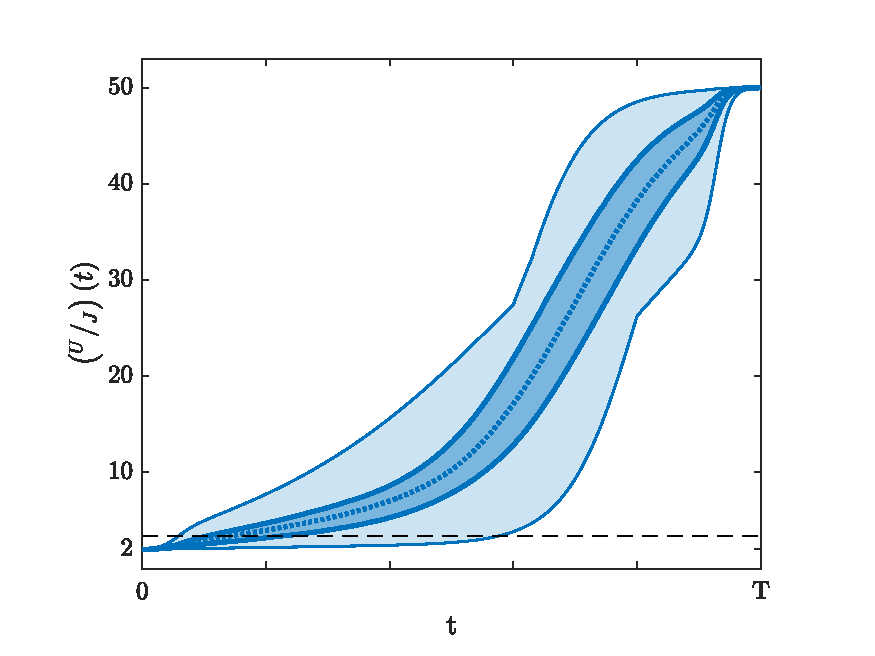
\includegraphics[width=0.7\textwidth]{Figures/LinSigSeed.pdf}
    \caption{\textit{Distribution of seeds used for optimization. All seeds lie within the lightly shaded region, while the darker region contains the 25-75 percentile of seeds. Lastly, the dotted line is the median value of the seed. The dashed line signifies the point of the Bose-Hubbard phase transition.}}
    \label{fig:LinSigSeed}
\end{figure}
Figure \ref{fig:LinSigSeed} shows the distribution of seeds used for the optimizations. Due to control parameter being the interaction strength of the Bose-Hubbard model, the phase transition occurs at quite a low value compared to the final value. Hence, the initial part of the seed is a slowly increasing linear ramp, which crosses the point of the phase transition with a small slope. A shape function has been multiplied to the seeds enforcing a horizontal slope at the start and end of the duration. This helps avoiding any kinks in the control curve, as the optimized part of the control is subjected to a shape function itself.


\subsection{Determining the Quantum Speed Limit}
To understand how the solutions area affected by the duration of the control sequence, a series of optimizations were made while scanning over the duration $T$. For this a regularization factor of $\gamma = 10^{-6}$ was used, while a medium optimization space dimension of $M = 20$ was used. Figure \ref{fig:FidelityDuration5} shows the final fidelities obtained for various durations from 100 different initial controls.
\begin{figure}[h!]
    \centering
    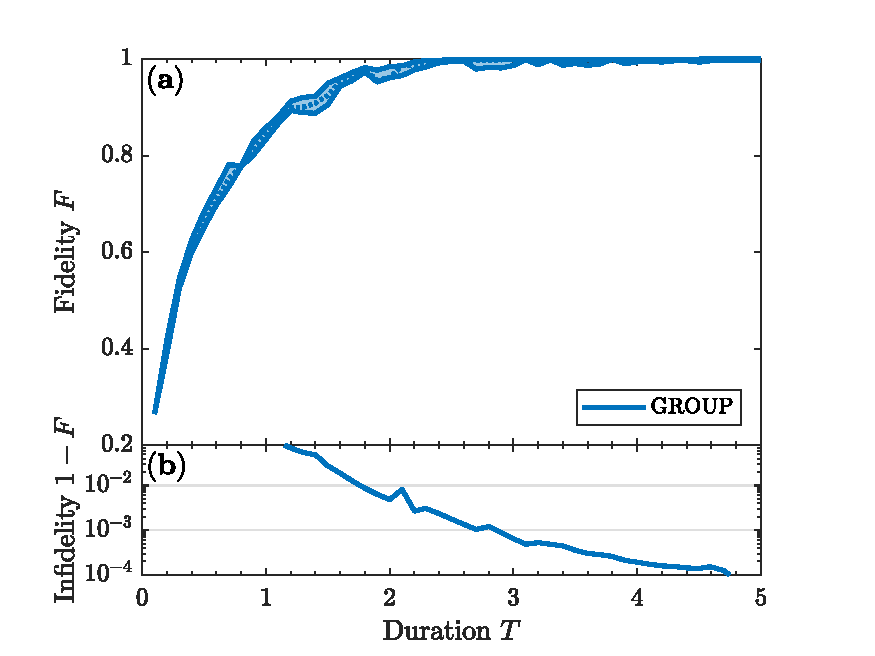
\includegraphics[width=0.8\textwidth]{Figures/5part/FidelityDuration.pdf}
    \caption{\textit{Final fidelity obtained for optimal control at various durations. \textbf{(a)} the dotted line marks the median fidelity achieved, while the shaded area displays the $25\%$- and $75\%$-quartiles of the solutions. \textbf{(b)} the lowest infidelity achieved for each duration. }}
    \label{fig:FidelityDuration5}
\end{figure}
In part \ref{fig:FidelityDuration5}.a the $25\%$- and $75\%$-quartiles along with the median of the solutions are displayed. At short durations the system can not evolve fast enough from the initial state to reach the target state, hence only low fidelities are obtained. However, as more and more time becomes available, fidelities very close to unit can be reached. Although the final fidelity does not appear to improve beyond $T=3$, figure \ref{fig:FidelityDuration5}.b reveals the best solutions improving at longer durations albeit at a much reduced rate. Due to the complexity of quantum states in lattice systems, achieving a perfect, unit fidelity is almost impossible. Therefore, a threshold for accepted final fidelity must be made in order to determine the quantum speed limit. Compared to other figures of merit, the fidelity is a very strong measure, as it only considers the overlap with the target state. Thus, at $I = 1-F = 10^{-2}$ $99\%$ of contributions to the final state comes the target state. MORE ABOUT QSL\\  
Furthermore, information regarding the control landscape as well as the consistency of the algorithm can be inferred from the spread in fidelities achieved. A large variety of final fidelities may be due to a control landscape with many local minima. On the other hand, the same phenomenon could be caused by the inability of an algorithm to accurately converge to the minimum. The interior point method is a very robust algorithm capable of handling non-linear constraints, whereby it is reasonable to assume the variations in solutions being caused by the underlying control landscape. Considering the fairly large variation in seeds shown in figure \ref{fig:LinSigSeed}, the control landscape of the 5-site problem must be relatively simple. NEED CONFIRMATION ON THIS.

\subsubsection{Best solutions at selected durations} 
